%%%%%%%%%%%%%%%%%%%%%%%%%%%%%%%%%%%%%%%%%12pt: grandezza carattere
                                        %a4paper: formato a4
                                        %openright: apre i capitoli a destra
                                        %twoside: serve per fare un
                                        %   documento fronteretro
                                        %report: stile tesi (oppure book)
\documentclass[12pt,a4paper,openright, oneside]{report}
%
%%%%%%%%%%%%%%%%%%%%%%%%%%%%%%%%%%%%%%%%%libreria per scrivere in italiano
\usepackage[italian]{babel}
%
%%%%%%%%%%%%%%%%%%%%%%%%%%%%%%%%%%%%%%%%%libreria per accettare i caratteri
                                        %   digitati da tastiera come è à
                                        %   si può usare anche
                                        %   \usepackage[T1]{fontenc}
                                        %   però con questa libreria
                                        %   il tempo di compilazione
                                        %   aumenta

\usepackage[T1]{fontenc}
\usepackage[utf8]{inputenc}
%
%%%%%%%%%%%%%%%%%%%%%%%%%%%%%%%%%%%%%%%%%libreria per impostare il documento
\usepackage{fancyhdr}
%
%%%%%%%%%%%%%%%%%%%%%%%%%%%%%%%%%%%%%%%%%libreria per avere l'indentazione
%%%%%%%%%%%%%%%%%%%%%%%%%%%%%%%%%%%%%%%%%   all'inizio dei capitoli, ...
\usepackage{indentfirst}
%
%%%%%%%%%libreria per mostrare le etichette
%\usepackage{showkeys}
%
%%%%%%%%%%%%%%%%%%%%%%%%%%%%%%%%%%%%%%%%%libreria per inserire grafici
\usepackage{graphicx}
\usepackage{float}
%
%%%%%%%%%%%%%%%%%%%%%%%%%%%%%%%%%%%%%%%%%libreria per utilizzare font
                                        %   particolari ad esempio
                                        %   \textsc{}
\usepackage{newlfont}
%
%%%%%%%%%%%%%%%%%%%%%%%%%%%%%%%%%%%%%%%%%librerie matematiche
\usepackage{amssymb}
\usepackage{amsmath}
\usepackage{latexsym}
\usepackage{amsthm}
%
\oddsidemargin=30pt \evensidemargin=20pt%impostano i margini
\hyphenation{sil-la-ba-zio-ne pa-ren-te-si}%serve per la sillabazione: tra parentesi 
					   %vanno inserite come nell'esempio le parole 
%					   %che latex non riesce a tagliare nel modo giusto andando a capo.

%
%%%%%%%%%%%%%%%%%%%%%%%%%%%%%%%%%%%%%%%%%comandi per l'impostazione
                                        %   della pagina, vedi il manuale
                                        %   della libreria fancyhdr
                                        %   per ulteriori delucidazioni
\pagestyle{fancy}\addtolength{\headwidth}{20pt}
\renewcommand{\chaptermark}[1]{\markboth{\thechapter.\ #1}{}}
\renewcommand{\sectionmark}[1]{\markright{\thesection \ #1}{}}
\rhead[\fancyplain{}{\bfseries\leftmark}]{\fancyplain{}{\bfseries\thepage}}
\cfoot{}
%%%%%%%%%%%%%%%%%%%%%%%%%%%%%%%%%%%%%%%%%
\linespread{1.3}                        %comando per impostare l'interlinea
%%%%%%%%%%%%%%%%%%%%%%%%%%%%%%%%%%%%%%%%%definisce nuovi comandi
%
\begin{document}
\begin{titlepage}                       %crea un ambiente libero da vincoli
                
%%%%%%%%%%%%%%%%%%%%%%%%%%%%%%%%%%%%%%%%
\clearpage{\pagestyle{empty}\cleardoublepage}%non numera l'ultima pagina sinistra
\end{titlepage}
\pagenumbering{roman}                   %serve per mettere i numeri romani

\chapter*{Introduzione}                 %crea l'introduzione (un capitolo
                                       %   non numerato)
%%%%%%%%%%%%%%%%%%%%%%%%%%%%%%%%%%%%%%%%%imposta l'intestazione di pagina
\rhead[\fancyplain{}{\bfseries
INTRODUZIONE}]{\fancyplain{}{\bfseries\thepage}}
\lhead[\fancyplain{}{\bfseries\thepage}]{\fancyplain{}{\bfseries
INTRODUZIONE}}
%%%%%%%%%%%%%%%%%%%%%%%%%%%%%%%%%%%%%%%%%aggiunge la voce Introduzione
                                        %   nell'indice
\addcontentsline{toc}{chapter}{Introduzione}

Le \textit{Security Token Offerings}, abbreviate in \textit{STOs}, sono un fenomeno recente che si è diffuso a partire dalla seconda metà del 2017 mantenendo inizialmente la connotazione di \textit{Initial Coin Offerings (ICOs)}, per poi prestare maggiore attenzione alla regolamentazione e differenziarsi in \textit{token sales} in cui il token è uno strumento finanziario regolamentato. 

Come si avrà modo di osservare, questo cambio di paradigma è ciò che contraddistingue le STOs. Nel 2017 le ICOs hanno raggiunto un picco di popolarità per poi la maggior parte fallire in meno di un anno, facendo capire agli investitori che le ICOs sono state una bolla speculativa. Nonostante ciò, la validità del modello di raccolta di capitale tramite la vendita di token basati su tecnologia Blockchain non è stata messa in discussione. Proprio per questo sono nate le STOs, delle token sales in cui il token è uno strumento finanziario, che offre tutela agli investitori. 

Lo scopo di questo lavoro di tesi è stato approfondire la comprensione di questo fenomeno in particolare analizzandone le motivazioni, le caratteristiche e le metodologie con le quali queste STOs vengono realizzate.

La tesi è strutturata come segue:
\begin{itemize}
    \item Nel primo capitolo si ripercorre la storia delle monete digitali per capire le complessità del processo di diffusione di queste. Vengono analizzate nel dettaglio le fasi della creazione e diffusione sia di Bitcoin che di Ethereum. Una volta comprese le motivazioni che hanno portato alla nascita di queste monete ne verrà considerata un'applicazione particolare, la raccolta di capitale. Di conseguenza, vengono confrontate le caratteristiche di diverse tipologie di token, in modo da poterli identificare e distinguere tra loro. 
    
    \item Nel secondo capitolo vengono presentati i protocolli principali con i quali le STOs vengono realizzate. Tra questi vengono prese in considerazione tre categorie principali. La prima categoria comprende lo standard ERC-20 e altri standard proprietari che estendono ERC-20. Nella seconda categoria vengono presentati gli standard dedicati a beni non fungibili, ovvero lo standard ERC-721 e il suo successore, lo standard ERC-1155. Infine, l'ultima categoria è lo standard ERC-1400 che comprende altri standard per i security tokens. 
    
    \item Nel terzo capitolo si discute dei principali driver di innovazione nel campo delle STOs. In primo luogo vengono presentate le IEOs, dei particolari tipi di token sales che avvengono su exchange dedicati.  Successivamente, si discute del ruolo di Libra, la criptovaluta proposta da Facebook, quale apripista per aprire un dialogo con i legislatori e stabilire un framework normativo chiaro. 
    
    \item Nel quarto capitolo vengono presentati i dati 
    ottenuti dopo una difficile ricerca. La difficoltà riscontrata è dovuta alla natura stessa delle STOs: le STOs si rivolgono esclusivamente ad investitori autorizzati, non ai consumatori. I dati presentati vengono poi analizzati per poter elaborare alcune considerazioni riguardo alle STOs. 
\end{itemize}

%%%%%%%%%%%%%%%%%%%%%%%%%%%%%%%%%%%%%%%%%non numera l'ultima pagina sinistra
\clearpage{\pagestyle{empty}\cleardoublepage} 

\tableofcontents                        %crea l'indice
%%%%%%%%%%%%%%%%%%%%%%%%%%%%%%%%%%%%%%%%%imposta l'intestazione di pagina
\rhead[\fancyplain{}{\bfseries\leftmark}]{\fancyplain{}{\bfseries\thepage}}
\lhead[\fancyplain{}{\bfseries\thepage}]{\fancyplain{}{\bfseries INDICE}}
%%%%%%%%%%%%%%%%%%%%%%%%%%%%%%%%%%%%%%%%%non numera l'ultima pagina sinistra
\clearpage{\pagestyle{empty}\cleardoublepage}
\listoffigures                          %crea l'elenco delle figure
%%%%%%%%%%%%%%%%%%%%%%%%%%%%%%%%%%%%%%%%%non numera l'ultima pagina sinistra
\clearpage{\pagestyle{empty}\cleardoublepage}
\listoftables                           %crea l'elenco delle tabelle
%%%%%%%%%%%%%%%%%%%%%%%%%%%%%%%%%%%%%%%%%non numera l'ultima pagina sinistra


\clearpage{\pagestyle{empty}\cleardoublepage}

\chapter{Differenze tra Initial Coin Offering e Security Token Offering}                %crea il capitolo
%%%%%%%%%%%%%%%%%%%%%%%%%%%%%%%%%%%%%%%%%imposta l'intestazione di pagina
\lhead[\fancyplain{}{\bfseries\thepage}]{\fancyplain{}{\bfseries\rightmark}}
\pagenumbering{arabic}
%mette i numeri arabi


\section{Storia delle monete elettroniche e delle cryptocurrency}

Sebbene le valute digitali abbiano raggiunto un nuovo livello di rilievo nel mondo solo negli ultimi anni, è importante ricordare che la monete elettroniche hanno una storia che risale a decenni fa. Il whitepaper “Bitcoin: A Peer-to-Peer Electronic Cash System”, pubblicato nel 2008 da un autore anonimo o da un gruppo di persone sotto lo pseudonimo di Satoshi Nakamoto, per quanto risulti innovativo e a posteriori anche rivoluzionario, si basa su tecnologie preesistenti e ben affermate tra le quali ad esempio le reti P2P, un fenomeno che ha radici nelle prime fasi della storia di Internet e reso popolare da Napster. Non sono solo le reti distribuite ad essere una fondazione per Bitcoin; nel whitepaper Nakamoto si avvale infatti di altri lavori precedenti che risultano fondamentali al funzionamento della rete. Tra questi possiamo citare il lavoro di tesi pubblicato da Ralph Merkle nei primi anni ’70  riguardo alla comunicazione sicura attraverso canali insicuri e gli sviluppi apportati da Diffie e Hellman. Inoltre, è proprio a Merkle che dobbiamo l’invenzione dei Merkle Tree usati in Bitcoin poiché forniscono un metodo per firmare digitalmente messaggi contenuti in grandi strutture dati. I merklee tree verranno successivamente ripresi da Bayer, Haber e Stornetta per la realizzazione efficiente di una catena di blocchi firmata crittograficamente.


Altri lavori più recenti risultano essere punti chiave per lo sviluppo della rete Bitcoin ed in generale dei sistemi di pagamento elettronici.


Nel 1983 in “Blind Signatures for Untraceable Payments” e nei sui lavori successivi, Chaum introduce l’idea di un sistema di pagamento elettronico anonimo basato sulla tecnologia di Blind Signature, sistema che verrà poi implementato dallo stesso autore con ECash™ nel 1994. Come osserva Schoenmakers nonostante le istituzioni finanziare già utilizzassero dietro le quinte sistemi elettronici per processare transazioni l’apertura al pubblico dei sistemi di pagamento elettronici introduce la necessità di un sistema di pagamento elettronico che possa essere utilizzato in una rete ad accesso pubblico, particolarmente in riferimento alla rete Internet. Nel 1998 DigiCash fallisce, principalmente a causa della forte competizione posta in atto dal sistema di pagamento tramite carta di credito. Nel particolare secondo Chaum la compagnia ha sofferto di un chicken-and-egg problem: fu difficile convincere abbastanza venditori  ad adottare il sistema per  poter acquisire clienti e vice versa. (Lo stesso destino spetta ad altre forme di pagamento elettronico dello stesso periodo tra le quali possono essere citate CyberCoin, Virtual PIN. ) 


Sebbene infruttuosa, l’esperienza di Chaum rappresenta il primo esempio di un sistema di pagamento elettronico anonimo e risulta pionieristico sia nei problemi che vengono presentati come nelle soluzioni proposte, come avviene nel caso del problema di double spending. 


Altri sistemi di moneta digitale si sono susseguiti negli anni, tra i più rilevanti possiamo citare e-gold, Liberty Reserve e PayPal: I primi due non più attivi, entrambi per controversie legali, mentre l’ultimo ancora attivo. Questa lista non ha scopo di essere esauriente, per un approfondimento si rimanda alla letteratura sull’argomento.
Un altro tassello fondamentale nello sviluppo delle monete elettroniche è l’introduzione nel 1997 di hashcash da parte di Adam Back che indipendentemente descrive un sistema simile a quanto proposto da Cynthia Dwork,  Moni Naor e Eli Ponyatovski nel 1992 in “Pricing via Processing or Combatting Junk Mail”. Entrambe le proposte prevedono l’utilizzo di quella che nel 1999 viene formalizzata da  Markus Jakobsson e Ari Juels come “proof of work” per arginare il fenomeno dello spam. Appena un anno prima, nel 1998, Wei Dai introduce B-money, un sistema basato su hashcash che comprendeva varie feature oggi comuni alla maggior parte delle cryptocurrencies. B-money tuttavia non fu mai lanciato e rimase solo una proposta ma il lavoro di Dai non fu vano; dieci anni dopo, all'inizio dello sviluppo di Bitcoin, Dai fu il primo ad essere contattato da Nakamoto. A lui seguirono altri sviluppatori tra i quali Nick Szabo, creatore di bitgold, e Hal Finney, che introdusse l'idea di "reusable PoW". 

Nel 1998 infatti, Nick Szabo creò bitgold, un meccanismo per una digital currency decentralizzata e sicura che implementava già alcune idee alla base degli smart contracts. Le teorie di Szabo riguardo riguardo gli accordi auto-attuanti furono formulato all'incirca durante lo stesso periodo in cui Ian Grigg introdusse l'idea dei Ricardian Contracts, un metodo per registrare un documento come un contratto legale e collegarlo in modo sicuro ad altri sistemi. Bitgold, come B-money, non fu mai implementato.
 
 Hal Finney nel 2004 introduce la prima Reusable PoW (RPoW), ancor prima della nascita di Bitcoin. Più tardi, nel 2009, Finney riceverà la prima transazione della rete Bitcoin, da parte di Nakamoto stesso. 

\subsection{Creazione e diffusione di Bitcoin}

La pubblicazione del whitepaper di Bitcoin avviene finalmente nel 2008, poco dopo il clou della crisi finanziaria e del collasso di Lehman Brothers. L'obbiettivo a cui Bitcoin mira è fornire una valuta digitale P2P che non necessiti della presenza di banche ed altri intermediari.  La prima implementazione di bitcoin fu opera di Nakamoto ma successivamente la direzione dei lavori passò gradualmente ad un gruppo di primi utenti e sviluppatori capitanati da Gavin Andersen. 

E' interessante notare come nel suo whitepaper Nakamoto non si riferisca a "blockchain" ma solo a "chain of blocks". Il termine "blockchain" infatti si diffonde successivamente durante lo sviluppo di protocolli alternativi a bitcoin. 

Dalla sua creazione nel 2008 fino ad oggi il prezzo di acquisto per un bitcoin è passato da  0.003\$, il valore della prima quotazione su un exchange dedicato, fino al valore massimo di circa 19000\$ come è possibile osservare nella figura \ref{fig:chartbitcoin}. A questo valore è stato stimato che il patrimonio di Nakamoto abbia raggiunto un valore di 19 miliardi di dollari, dato che possiede circa un milione di bitcoin, o più. Nonostante ciò, dalla sua uscita di scena nel 2011 Nakamoto non ha operato transazioni con i bitcoin di cui sappiamo essere in possesso. 
\begin{figure}[H]
  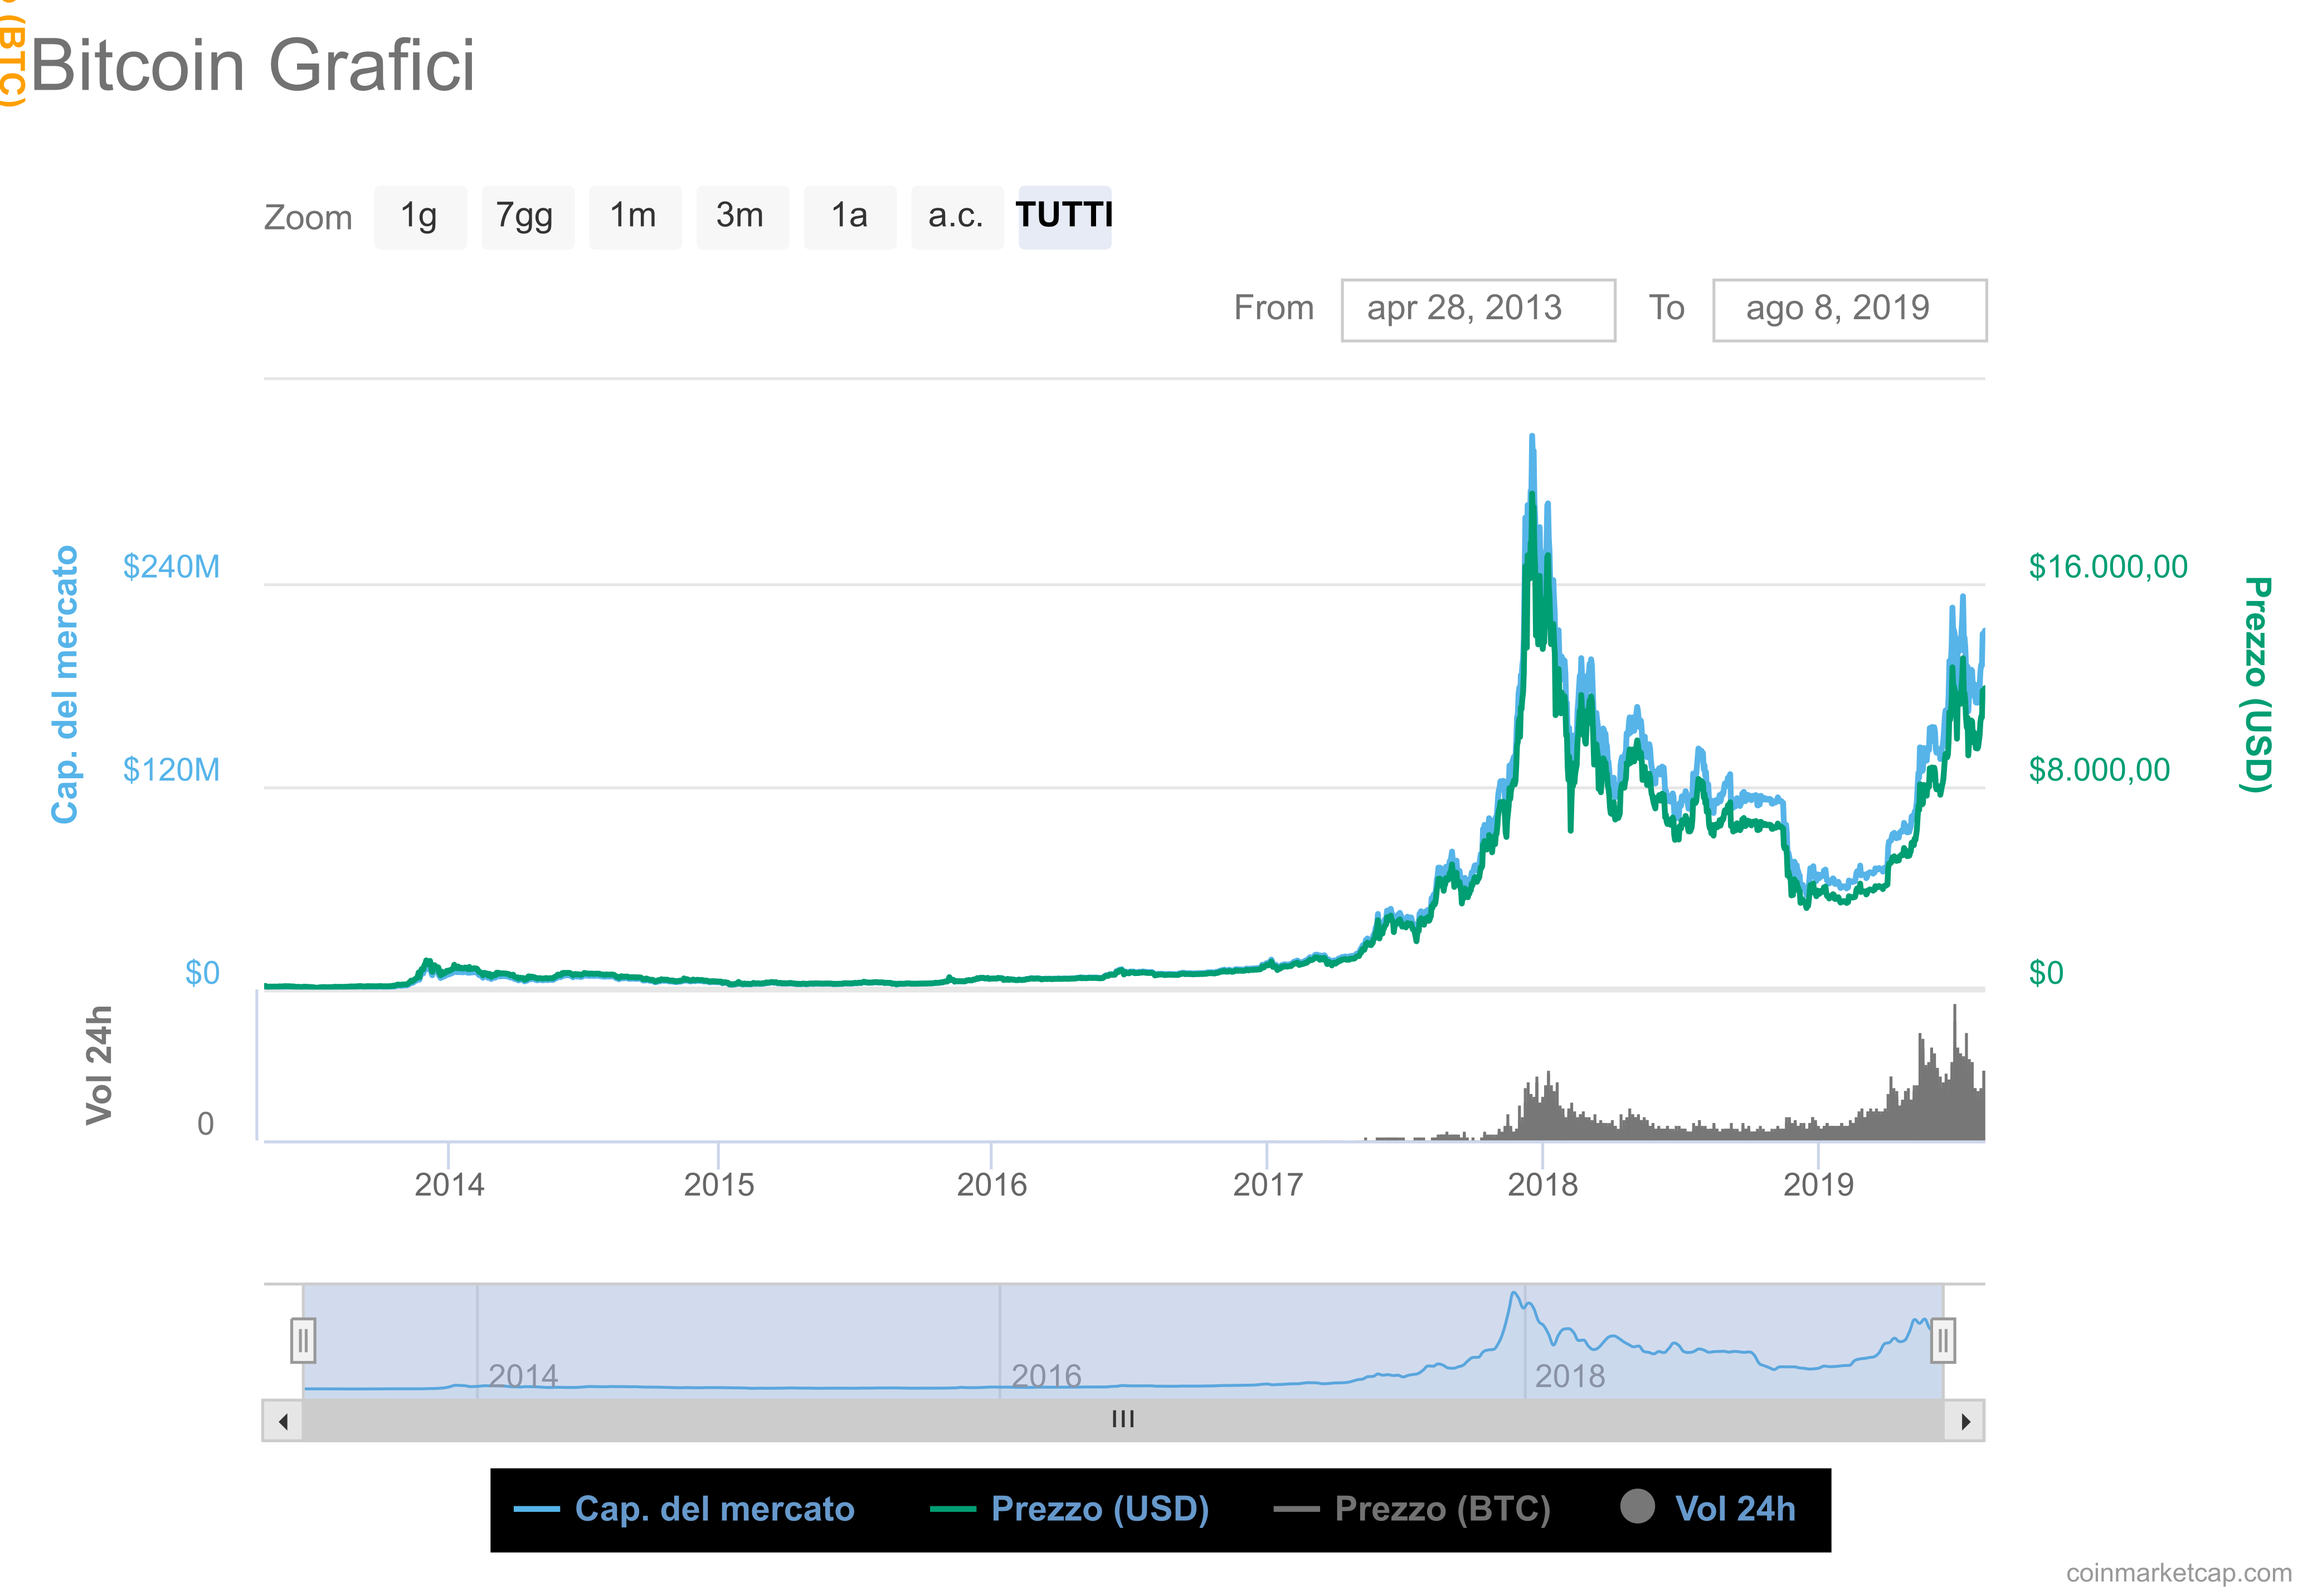
\includegraphics[width=\linewidth]{chartbitcoin.png}
  \caption{Bitcoin price chart}
  \label{fig:chartbitcoin}
\end{figure}

Il codice open source di Bitcoin ha permesso ad altri sviluppatori di creare protocolli alternativi (Chohan 2017e), in questo periodo infatti si assiste alla nascita di quelle che verranno in seguito definite "Altcoin", un'abbreviazione di "alternative coin". Allo stesso tempo si inizia a diffondere anche l'utilizzo di Bitcoin in alcune organizzazioni, tra le prime possiamo citare Wikileaks e Electronic Frontier Foundation. Nel 2011 viene pubblicato il sito tematico Bitcoin Magazine che tra i suo fondatori annovera anche Vitalik Buterin. Nel 2012 la Bitcoin Foundation inizia i propri sforzi di standardizzazione e promozione di Bitcoin. Nello stesso anno BitPay, un azienda che offre servizi di pagamento tramite bitcoin riporta che più di 1000 commercianti avevano adottato il suo sistema di pagamento. Nel 2013, Coinbase, un'altra azienda per il processo dei pagamenti tramite bitcoin, annuncia di aver venduto bitcoin per un valore pari a 1 milione di dollari in un mese, ad un prezzo di circa 22\$ per unità. 
A questo punto, l'utilizzo di bitcoin entra nei radar degli enti regolatori a causa di una alta volatilità dovuta a diversi fattori concorrenti. L'American Financial Crimes Enforcement Network (FinCEN) stabilisce delle linee guida per monete virtuali decentralizzate, con particolare riferimento a Bitcoin, introducendo l'obbligo per i miners di essere registrati come Money Service Business (MSBs) qualora vendessero i bitcoin generati. Anche altri enti americani entrano in contatto con bitcoin durante incidenti ed indagini, come ad esemplificato da un avviso di sequestro emesso dalla Drug Enforcement Agency (DEA) per 11 bitcoins. Non a caso, a partire dal 2013 si può osservare una divergenza nelle regolamentazioni implementate da diversi stati. 
Tra gli esempi più rilevanti possiamo citare il caso tailandese: il Foreign Exchange Administration and Policy Department sancisce che il bitcoin è illegale data l'assenza di un framework legale al quale possa essere sottoposto. Nel frattempo, il giudice federale amos Mezzant del distretto est del Texas riconosce i bitcoins come "una moneta o una forma di moneta" come definito dalle Federal Securities Laws. Verso l'ottobre del 2013, l'FBI sequestra 26000 bitcoins, per un valore di circa 3,6 milioni di dollari, durante l'arresto di Ross William Ulbricht, creatore del sito Silk Road, un sito di commercio elettronico che si avvaleva di bitcoin e dedicato al contrabbando. Il 2013 risulta essere un anno saliente per bitcoin anche per un altro aspetto. La Cina diventa infatti il più grande punto di scambio di bitcoin. Tuttavia la Banca Popolare Cinese (PBC o PBOC) proibisce l'uso di bitcins agli istituti finanziari cinesi, cusando in dicembre un crollo dei prezzi. 

Nel 2014 emergono prodotti derivati basati su Bitcoin, approvati dall'U.S.Commodity Futures Trading Commission come prodotti di scambio over-the-counter che hanno come sottostante il prezzo del bitcoin. Inoltre, aumentano i casi di furto elettronico di bitcoin, di particolare rilievo risultano essere i casi di Mt Gox e Bitstamp. 
Da qui in poi l'espansione globale di Bitcoin continua inesorabilmente, nonostante le incertezze della mutevole configurazione giuridica nei diversi stati, grazie anche ad una tendenza di regolamentazione più favorevole.  

\subsection{Creazione e diffusione di Ethereum}

Ethereum viene descritto in un whitepaper da Vitalik Buterin, verso la fine del 2013.
Vitalik riporta che durante l'ottobre del 2013 lavorando in Israele a contatto con il team di Mastercoin, in "Utimate Scripting" avanza delle proposte per generalizzare il protocollo utilizzato da Mastercoin. Queste proposte risultano abbastanza distanti dalle funzionalità di Ethereum, rappresentano infatti una prima versione di un protocollo finalizzato solo alla creazione di un contratto tra due parti nelle quali il valore monetario viene redistribuito secondo una formula specificata nel contratto stesso. Sebbene impressionato, il team di Mastercoin decise di non implementare le modifiche proposte. In Dicembre Buterin propone una nuova versione, la prima che adotta il nome Ethereum e che presenta una generalizzazione degli smart contracts. In questa versione infatti invece di utilizzare un linguaggio di scripting per descrivere i termini di una relazione tra due parti, gli smart contracts sono account veri e propri, con la possibilità di possedere, spedire e ricevere assets. Da questo momento in poi Ethereum attira l'interesse di altri sviluppatori, primi tra i quali Gavin Wood, Jeffrey Wilcke, Andrew Miller, Mihai Alisie, Anthony Di Iorio e Charles Hoskinson. 
Ethereum viene formalmente annunciato il 25 Gennaio 2014 a Miami durante la North America Bitcoin Conference  e nell'estate del 2014 dopo i primi lavori degli sviluppatori il protocollo si stabilizza, quindi Wood pubblica una specifica semi-formale di Ethereum e dell'Ethereum Virtual Machine. Intanto altri sviluppatori si aggiungono al progetto ed anche alcuni finanziatori decidono di prendervene parte.
Parallelamente a queste prime fasi di sviluppo vengono formate diverse entità legali per poter coordinare il progetto, in particolare Ethereum Switzerland GmbH (EthSuisse) e Ethereum Foundation (Stiftung Ethereum). Lo svilippo fu finanziato tramite crowdfounding, vendendo il token di ethereum, denominato ether, in cambio di bitcoin. Grazie alla crowdsale, 11,9 milioni di ether furono venduti, per un valore di circa 18,4 milioni di dollari. 

Sin dal suo lancio iniziale, Ethereum ha ricevuto numerosi aggiornamenti pianificati del proprio protocollo, con cambiamenti importanti per quanto riguarda le funzionalità dello stesso. 
A testimonianza del successo del progetto Ethereum, nel marzo 2017, varie startups, gruppi di ricerca e aziende appartenenti alla Fortune 500 hanno annunciato la creazione della Enterprise Ethereum Alliance (EEA) con trenta membri fondatori. 
In maggio, l'organizzazione no-profit conta 116 membri, includendo ConsenSys, CME Group, Cornell University's research group, Toyota Research Institute, Samsung SDS, Microsoft, Intel, J. P. Morgan, Cooley LLP, Merck KGaA, DTCC, Deloitte, Accenture, Banco Santander, BNY Mellon, ING, and National Bank of Canada.
In Luglio il numero di membri raggiunge i 150, tra i quali MasterCard, Cisco Systems, Sberbank and Scotiabank. Altri membri di rilevo sono Advanced Micro Devices (AMD), FedEx Corporate Services, Hyperledger, Securitize, TOKENY, UniCredit e VMware.

\section{Le cryptocurrencies come strumento di finanziamento}
Come già accennato, inizialmente Ethereum ricevette finanziamenti tramite una crowdsale sulla rete Bitcoin.  Questo ha permesso agli sviluppatori di intercettare l'interesse degli utenti disposti a supportare lo sviluppo della piattaforma. Tuttavia, la prima token sale avvenne nel luglio 2013 grazie a J.R. Willett con lo scopo di raccogliere fondi per il progetto Omni tramite la vendita di Mastercoin. Per motivare i potenziali investitori a contribuire al progetto, Willet fece in modo di rendere disponibile molte delle funzioni solo ai possessori di mastercoins. Fu quindi Willet ad ideare il modello delle ICO ed a lui dobbiamo anche l'introduzione di quelli che successivamente verranno definiti come utility token. La token sale permise a willet di raccogliere finanziamenti per un valore di 600 mila dollari, al tempo circa 4740 bitcoin. Il protocollo introdotto con mastercoin, oggi chiamato "Omni Layer", ha avuto molto successo tanto da essere usato come protocollo su cui si basa il token Tether (USDT), ad oggi una delle cryptocurrencies più scambiate dopo il bitcoin. 
Il secondo token venduto tramite ICO è NextCoin (NXT), che tra settembre ed ottobre del 2013 permette al suo creatore, rimasto anonimo, di raccogliere 21 bitcoin, per un valore compreso tra i 3000 e 17000 dollari. A NextCoin seguono Counterparty (XCP), MaidSafeCoin (MAID), Swarm e successivamente Ethereum. 

Poiché Ethereum è pensata come una piattaforma per la creazione ed esecuzione di smart contract e grazie alla possibilità di sviluppare token sulla piattaforma stessa, risulta ovvio il perché Ethereum sia diventata la piattaforma più usata per ospitare altre crowdsale. La prima Initial Coin Offering (ICO) basata sulla piattaforma Ethereum fu lanciata il 17 Agosto 2015, per la vendita di token Augur. La vendita durò fino al 5 Settembre dello stesso anno. In seguito alla vendita vennero raccolti più di 5 milioni di dollari per lo sviluppo del progetto Augur. Il progetto è stato lanciato ufficialmente nel luglio del 2018. 

Il fenomeno delle ICO è via via diventato popolare con un picco nel 2017. Dall'inizio  del 2017 fino ad ottobre 2017 infatti,  vengono raccolti fondi per un valore di 2,3 miliardi di dollari, un risultato dieci volte maggiore rispetto al 2016. 
Durante tutto il 2017 vengono raccolti fondi per un valore di circa 6 miliardi di dollari, il 37\% dei quali dovuti a solamente 20 ICO. 
Viene stimato che al Febbraio 2018 il 46\% delle progetti finanziati tramite un'ICO nel 2017 sono falliti. 
 
https://en.wikipedia.org/wiki/Initial coin offering

\section{Classificazione dei token nelle token sales}
\subsection{Il modello delle Initial Coin Offerings}
Nelle ICO possono essere identificate varie caratteristiche per classificare un token, prima tra tutte la sua funzione. Comunemente, in base alla sua funzione, un token può essere considerato un utility token, un security token o un currency token. Questa distinzione è comunemente riconosciuta ed è adottata anche dalla Swiss Financial Market Supervisory Authority (FINMA). 

In questo caso assumiamo che il termine token si riferisca alla rappresentazione digitale tramite blockchain di un asset.

Un currency token, come ad esempio il bitcoin, rappresenta una valuta digitale e sono un mezzo di scambio.
Un utility token è usato all'interno di una rete per poter accedere ad una funzionzionalità o per il funzionamento di questa. 
In modo simile a quanto già detto sui token, i security tokens si riferiscono ad una rappresentazione digitale tramite blockchain di securities. La definizione di security tuttavia varia a seconda della legislazione applicabile. Negli Stati Uniti le securities sono definite nell'U.S. Code of Laws 15 §77b(a)(1) come:
The term ‘‘security’’ means any note, stock, treasury stock, security future, bond, debenture, evidence of indebtedness, certificate of interest or participation in any profit sharing agreement, collateral-trust certificate, preorganization certificate or subscription, transferable share, investment
contract, voting-trust certificate, certificate of deposit for a security, fractional undivided interest in oil, gas, or other mineral rights, any put, call, straddle, option, or privilege on any security, certificate of deposit, or group or index of securities (including any interest therein or based on the value thereof), or
any put, call, straddle, option, or privilege entered into on a national securities exchange relating to foreign currency, or, in general, any interest or instrument commonly known as a ‘‘security’’, or any certificate of interest or participation in, temporary or interim certificate for, receipt for, guarantee of,
or warrant or right to subscribe to or purchase, any of the foregoing.”

Invece in Italia l'equivalente delle securities sono gli strumenti finanziari definiti nel D.lgs 24 febbraio 1998 n.58, noto come testo unico della finanza, abbreviato TUF, o anche legge Draghi. 


https://www.investopedia.com/terms/h/howey-test.asp



\subsection{Il modello delle Security Token Offerings}
Le Security Token Offerings (STOs) sono l'evoluzione naturale delle ICO. Questa evoluzione è dovuta alla necessità per le aziende di operare nel settore delle cryptocurrencies definendo con chiarezza le normative da rispettare. Lo scopo delle STOs infatti è esclusivamente quello di creare token equiparabili a securities. In questo modo, configurandosi come securities, viene aggirato il vuoto normativo o l'incompletezza legislativa ancora presente in vari stati. è infatti vantaggioso per un azienda trattare un token come una securietis poiché ci si configura in un ambito normativo già consolidato e di cui molti professionisti hanno già esperienza. Questo approccio si basa sull'idea che una securities non è definita dal mezzo con la quale essere viene rappresentata, ponendo quindi un'equivalenza tra un documento cartaceo e uno digitale.  Da questo punto di vista l'approccio comunemente adottato è quello di operare in una singola legislazione oppure operare in legislazioni diverse facendo attenzione a soddisfare ai requisiti imposti. Quest'ultimo caso richiede uno sforzo nettamente maggiore rispetto al primo; Operando in una sola legislazione è possibile gestire la maggior parte dei requisiti in modo automatico, o molto agevolato, attraverso l'implementazione di uno smart contracts dedicato. Operando in legislazioni diverse, l'implementazione dello smart contract deve essere compatibile per più legislazioni con il rischio di essere troppo generico o troppo specifico. In entrambi i casi non è ancora presente un meccanismo di automatic compliance. Alla singola azienda è quindi richiesto di occuparsi della burocrazia e della documentazione legalmente richiesta. Allo stesso tempo è compito dell'azienda assicurarsi di essere autorizzata all'emissione di securities. Ovviamente il maggiore sforzo richiesto all'issuer della securities si traduce in un maggiore costo rispetto ad un ICO. Tuttavia, il maggiore costo permette all'azienda di ridurre il rischio di contenziosi legali e di evitare la possibilità di sanzioni. 

http://www.scirp.org/journal/paperinformation.aspx?paperid=93164

In a recent paper (2019), Ante & Fielder [24] compare STOs with ICOs and share the opinion that “offerings of security tokens promise to better fit firms’ and investors’ needs and fill the role that ICOs failed to meet”. They mention several expected advantages of security tokens over traditional stocks: they are immediately transferable, they can be traded 24/7 on secondary markets, they no longer require brokers and custody accounts, and their underlying blockchain ensures the transparency and security of transactions.


https://alphapoint.com/wp-content/uploads/2019/08/Tokenized-Security-Commercial-Real-Estate.pdf


 They share the same legal constructs as traditional securities but often enable additional technical features (such as automatic
payments, transparent ownership history, and immutable ownership record) by
virtue of being on the blockchain. To date, the U.S. CFTC, IRS, and SEC have provided
some guidance around the status of digitally represented assets, but ambiguity
remains.
In the U.S., the Howey test is a test used to determine whether certain transactions
qualify as ‘investment contract’. If so, the transaction falls under securities law and is
therefore subject to the regulatory oversight of the SEC. The offer, sale, and
distribution of securities is regulated in the U.S. and requires registration of both the
security and the venues on which that security trades or to qualify for an exemption
from registration. Recent SEC “Framework for ‘Investment Contract’ Analysis of
Digital Assets” provides detailed guidance on the application of the Howey Test to
5
digital assets. According to the framework, an investment contract exists when there
is the investment of money in a common enterprise with a reasonable expectation
of profits to be derived from the efforts of others. These are the four prongs of Howey
Test: 1)The Investment of Money 2)Common Enterprise 3)Reasonable Expectation of
Profits 4) Derived from Efforts of Others
It is important to note that securities regulation is typically technology agnostic.
Anything that represents a security (whether a piece of paper, a record in a database,
or a token on a blockchain) that is bought or sold falls by legal definition under
securities law. Thus, "security token" is a token (technology implementation) that
acts as a security (legal concept).
Other non-U.S. jurisdictions have issued guidance on their definitions of various
types of tokens; however, differences exist depending on jurisdiction and different
uses in terminology abound. Two examples below are from the Financial Conduct
Authority (FCA), UK guidance from January, 2019 and the Swiss Financial Market
Supervisory Authority (FINMA) guidance from February, 2018. They have primarily
distinguished between ‘utility token’ and ‘security / asset token’:
 UK Financial Conduct Authority (2019):
“Security tokens are tokens with specific characteristics that mean they meet
the definition of a Specified Investment like a share or a debt instrument as
set out in the Regulated Activities Order, and are within the perimeter.
While, utility tokens grant holders access to a current or prospective product
or service but do not grant holders rights that are the same as those granted
by Specified Investments.”
6
Swiss Financial Market Supervisory Authority (2018):
“Asset tokens represent assets such as participations in real physical
underlyings, companies, or earnings streams, or an entitlement to dividends
or interest payments. In terms of their economic function, the tokens are
analogous to equities, bonds or derivatives.
While, Utility tokens are tokens which are intended to provide digital access
to an application or service.”

Security Tokens vs. Tokenized Security
We believe it is important to make a distinction between two types of
blockchain-based representations of securities: “security tokens”, which are
blockchain-native tokens are securities but do not exist outside of the blockchain,
versus “tokenized securities”, which are blockchain-embedded representations of
real world securities.
Both security tokens and tokenized securities can confer benefits over traditional
means of representing securities, such as on paper, or digitally in siloed databases.
However, they differ largely in the type of legal and regulatory frameworks they may
require to achieve impactful adoption. Settlement finality is one example. Finality
refers to a transaction being considered ‘final’ and it cannot be unwound. It is crucial
that any transfer of payment or transfer of ownership of an asset has finality and is
binding on both parties. As per the DTCC white paper titled ‘Guiding Principles for
8
the Post-Trade Processing of Tokenized Securities’, the point at which settlement
becomes final is determined by both the rules of the market (operational finality)
and the governing legal framework in the relevant jurisdiction (legal finality).
Operational finality concerns would arise for both native and embedded securities
and would be dependent on the consensus mechanism of the underlying
blockchain. However, a framework to confer legal finality to the transfer of
cryptographic keys may be needed to support the use of blockchain native
securities. On the other hand, with tokenized securities, where existing processes are
augmented using blockchain-based systems to represent securities during some or
all points of the transfer of ownership process, clarity around legal finality is often
aligned with current definitions
The differences between security tokens and tokenized securities are outlined in the
table below. Our research focuses primarily on tokenized securities given that many
viable blockchain projects today augment rather than entirely replace the traditional
market infrastructures for securities.
Security Token vs. Tokenized Security
Security Token Tokenized Security
Blockchain native Blockchain embedded
Token represents a security that doesn’t
exist outside of the blockchain (DAO,
collateralized crypto loan, etc.)
Token represents a security that exists
independent from a blockchain
(Tokenized equity, debt, etc)
To date, security tokens have imitated
traditional securities, although there is
potential for disruption when structured
products are layered on top
Traditional security achieves additional
features (positive or negative) by being
represented by a token, such as
automatic payments
Similar to ‘Bearer asset’ Similar to ‘Depository receipt’
Tokenized Security vs. Tokenized Asset
Security tokenization is a subset of asset tokenization (all securities are assets but
not all assets are securities). Our work focuses on the tokenization of securities that
have reference to underlying real assets, specifically commercial real estate. For
example, tokenization of an asset such as a land title is a tokenized asset, as opposed
to the tokenization of an equity or debt share.


https://doi.org/10.2139/ssrn.3356303

https://decrypt.co/5311/security-token-offerings-advantages

\chapter{Confronto tra le implementazioni}
Nel corso degli ultimi anni la community di sviluppatori ha portato avanti diverse iniziative per imporre uno standard condiviso per le security token offering. Inizialmente lo standard de facto è stato ERC-20\cite{K37}, già ampiamente adottato dalla maggior parte delle Initial coin Offering. Tra gli standard utilizzati per le STO, ERC-20 è lo standard più maturo e con maggiore supporto essendo stato creato verso la fine del 2015. Altri tentativi di standardizzazione nascono dalla necessità di garantire all'issuer della security token offering una maggiore governance e per facilitare il rispetto delle regolamentazioni sulle securities. Non a caso infatti possiamo osservare come molti tentativi di standardizzazione siano stati operati da aziende che offrono piattaforme per il token issuing. Per la maggior parte di queste aziende l'approccio è stato quello di estendere lo standard ERC-20, in modo da ottenere retrocompatibilità ed essere più appetibili alla community di sviluppatori con conoscenza dello standard sopracitato. Tra i casi che verranno analizzati troviamo: 
\begin{itemize}
    \item ST-20\cite{K38}, sviluppato da Polymath
    \item R-Token\cite{K39}, sviluppato da Harbor
    \item DS Protocol\cite{K41}, sviluppato da Securitize
    \item T-REX\cite{K42}, sviluppato da Tokeny
    \item S3\cite{K43}, sviluppato da OpenFinace
\end{itemize}

Altri standard si sono sviluppati a partire da necessità diverse, come nel caso degli standard ERC-721 ed ERC-1155 che implementano token non fungibili. La notorietà di questi protocolli è in parte dovuta all'introduzione del concetto di scarsità digitale tramite l'utilizzo di token non omogenei, un approccio che ben si presta all'ambito videoludico. 
Una proposta più recente e che ha ottenuto maggiore supporto sia dalla community sia da aziende, alcune delle quali già in possesso di uno standard proprietario, è lo standard ERC-1400, rinominato Security Token Standard\cite{K45}. ERC-1400 è una collezione di diversi standard sviluppati per essere interoperabili e facilmente estendibili all'emergere della necessità di nuove funzionalità da introdurre. Il passaggio ad uno standard condiviso e supportato da più stakeholder rappresenta uno step fondamentale par la diffusione di questo fenomeno.

\section{Implementazione con token ERC-20}
ERC-20 definisce un'interfaccia standard che rappresenta un token. Lo standard fornice funzionalità basilari per il trasferimento dei token. Lo scopo principale dello standard è quello di permettere interoperabilità tra le applicazioni che supportano lo standard, come ad esempio wallets ed exchanges. 
Lo standard ERC-20 prevede le seguenti funzioni:
\begin{lstlisting}[language=Solidity,numbers=none]
totalSupply() public view returns (uint256 totalSupply)
\end{lstlisting} 
\begin{lstlisting}[language=Solidity,numbers=none]
balanceOf(address _owner) public view returns (uint256 balance)\end{lstlisting}
\begin{lstlisting}[language=Solidity,numbers=none] 
transfer(address _to, uint256 _value) public returns (bool success)\end{lstlisting} 
\begin{lstlisting}[language=Solidity,numbers=none]
transferFrom(address _from, address _to, uint256 _value) public returns (bool success)
\end{lstlisting}
\begin{lstlisting}[language=Solidity,numbers=none]
approve(address _spender, uint256 _value) public returns (bool success)
\end{lstlisting}
\begin{lstlisting}[language=Solidity,numbers=none]
allowance(address _owner, address _spender) public view returns (uint256 remaining)
\end{lstlisting}
Inoltre, vengono definiti i seguenti eventi:
\begin{lstlisting}[language=Solidity,numbers=none]
Transfer(address indexed _from, address indexed _to, uint256 _value)
\end{lstlisting}
\begin{lstlisting}[language=Solidity,numbers=none]
Approval(address indexed _owner, address indexed _spender, uint256 _value)
\end{lstlisting}
Due delle implementazioni più diffuse di questo standard sono state realizzate da OpenZeppelin e ConsenSys. Le due implementazioni sono entrambe pienamente compatibili con lo standard sebbene presentino delle lievi differenze come si può osservare in appendice \ref{appendix:ERC-20Interface}.

Una appunto interessante si può trarre osservando i cambiamenti avvenuti durante lo sviluppo iniziale dello standard. Se in principio le prime bozze dello standard prevedevano un focus sulla creazione di "Coin", gli sviluppatori in modo lungimirante hanno deciso di generalizzare il protocollo per renderlo applicabile ad ogni bene fungibile trasferibile, motivo per il quale è stata scelta la denominazione più generica di "token"\cite{https://www.reddit.com/r/ethereum/comments/3n8fkn/lets_talk_about_the_coin_standard/}.

\subsection{ERC-20 proprietary extension}
\subsubsection{ST-20}
Lo standard ST-20 introdotto da Polymath nasce con l'obbiettivo di aggiungere all'interfaccia ERC20 la possibilità di inserire restrizioni allo scambio di token in modo da poter essere conforme alle normative sulle securities. 
In appendice \ref{appendix:ST20} è possibile osservare l'interfaccia dello smart contract che definisce un security token che rispetta lo standard ST-20. Trattandosi di un'estensione, lo smart contract è compatibile con lo standard ERC-20 e ne implementa tutte le funzioni e gli eventi previsti, aggiungendo a questi altre funzionalità e caratteristiche che agevolano l'adattabilità e la governance della STO. Per esempio, nel caso dello scambio senza restrizioni tra due parti, un caso che non sempre è desiderabile nelle STO, le transazioni possono essere limitare da una funzione "verifyTransfer". Ciò permette inoltre l'implementazione di una whitelist, una blacklist, un limite minimo/massimo di trasferimento, etc. 
In modo più dettagliato, l'interfaccia creata da Polymath si avvale principalmente di tre tipi componenti: un primo tipo detto "Transfer Manager", un tipo di moduli denominati "permission modules" e infine un modulo che si occupa delle funzionalità della token sale, ovvero, gli "STO modules". 
L'utilizzo di numerose componenti per implementare diverse funzionalità permette di avere un architettura modulare che comprende di volta in volta solamente le funzionalità richieste, permettendo così di rendere lo smart contract più efficiente.

\subsubsection{R-Token}
R-token, implementat da Harbor offre delle caratteristiche che lo rendono particolarmente innovativo, tanto da essere concettualmente compatibile con un token ERC-1400.Un altro aspetto particolare del protocollo è l'integrazione di una whitelist per gli exchange presenti nell'ecosistema proposto da Harbor. 
R-Token, che sta per "regualted token" si differenzia dagli altri standard compatibili con ERC-20 D<per l'adozione di alcuni servizi di document management e di custody. 
Generalmente una STO Harbor si compone di tre smart contracts;
\begin{itemize}
    \item Un "Regulator Service" che si occupa di interagire tramite un oracolo con la regolamentazione definita off.chain. 
    \item Un "Service Registry" che contiene un riferimento al "Regulator Service". Questo riferimento può essere modificato per permettere di aggiornare la business logic della STO. 
    \item Uno smart contract "R-Token" che contiene le caratteristiche del token, le sue funzioni e un riferimento immutabile al "Service Registry"
\end{itemize}
\subsubsection{DS Protocol}
L'estensione di ERC-20 proposta da Securitize ha due componenti principali. Il primo è lo smart contract "DSTokenInterface" che nel complesso non risulta apportare cambiamenti rilevanti rispetto ai protocolli già presentati. Il secondo componente risulta essere più originale ed è lo smart contract "DSServiceConsumerInterface" definito come segue:
\begin{lstlisting}[language=Solidity,numbers=none]
function getDSService(uint _serviceId) public view returns (address);

function setDSService(uint _serviceId, address _address) public /*onlyMaster*/ returns (bool);
\end{lstlisting}
queste funzioni permettono l'associazione dinamica di componenti e di verificare la presenza componenti  in modo dinamico (al fine di mantenere compatibilità tra diverse versioni del protocollo). I servizi sono identificati da un id nel seguente modo:
\begin{lstlisting}[language=Solidity,numbers=none]
 uint public constant TRUST_SERVICE = 1;
 uint public constant DS_TOKEN = 2;
 uint public constant REGISTRY_SERVICE = 4;
 uint public constant COMPLIANCE_SERVICE = 8;
 uint public constant COMMS_SERVICE = 16;
 uint public constant WALLET_MANAGER = 32;
 uint public constant LOCK_MANAGER = 64;
 uint public constant ISSUANCE_INFORMATION_MANAGER = 128;
 \end{lstlisting}
\subsubsection{T-REX}
T-REX, per esteso "Token for Regulated EXchanges", Presenta un approccio diverso rispetto ad altri protocolli. L'identità infatti ricopre un ruolo fondamentale nel protocollo, tanto da prevedere dei meccanismi di gestione dell'identità dell'investitore on-chain secondo i protocolli ERC-725 ed ERC-735. Il meccanismo di controllo dell'identità sostituisce la logica di whitelisting e blacklisting rendendo il protocollo più flessibile. Possiamo osservervare il funzionamento del protocollo nel seguente diagramma: 

\subsubsection{S3}
https://medium.com/openfinance/openfinance-network-smart-security-standard-s3-contract-270e7e4f4d22


\section{Implementazione con token ERC-721 e ERC-1155}
http://erc721.org/
https://www.cryptoclubitalia.it/enjin-token-erc-1155-videogiochi/
\section{Implementazione con token ERC-1400}
https://github.com/ConsenSys/ERC1400
https://blog.polymath.network/erc1400-implementation-approach-c668c4fbf40
https://github.com/bokkypoobah/SecurityToken
\subsection{ERC-1410: Partially Fungible Token Standard}
https://github.com/ethereum/EIPs/issues/1410
\subsection{ERC-1594: Core Security Token Standard}
https://github.com/ethereum/EIPs/issues/1594
\subsection{ERC-1643: Document Management Standard}
https://github.com/ethereum/EIPs/issues/1643
\subsection{ERC-1644: Controller Token Operation Standard}
https://github.com/ethereum/EIPs/issues/1644
\subsection{ERC-2258: Custodial Ownership Standard}
https://github.com/ethereum/EIPs/issues/2258
\section{Implementazione in altre blockchain}
\subsection{SRC20}
https://www.swarm.fund/src20
\subsection{Stellar}
https://medium.com/quillhash/ethereum-or-stellar-which-platform-is-best-suitable-for-your-ico-sto-7f1368bb942c
\subsection{EOS}
https://stoupdates.com/eos-enters-the-security-token-scene-with-the-launch-of-new-protocol/
\subsection{Hyperledger}
\subsection{Corda}
https://stowise.com/company/r3/
\subsection{Tezos}
https://www.reddit.com/r/tezos/comments/cdl2bu/tezos_explainer_3_reasons_why_tezos_is_the_best/
\subsection{NEO}
https://www.securities.io/neo-announces-formation-of-security-token-industry-consortium/
\subsection{Tron}
\section{Considerazioni sulle implementazioni}

https://info.binance.com/en/research/marketresearch/tokenization.html SUPER IMPORTANT

https://medium.com/atomic-capital/state-of-the-standards-a-technical-review-of-current-digital-securities-standards-3bc79f5aaf73
https://medium.com/@ElectricCapital/electric-capital-developer-report-h1-2019-7d836d68fecb

\clearpage{\pagestyle{empty}\cleardoublepage}

\chapter{Sviluppi futuri delle STOs}
\section{Initial Exchange Offerings (IEOs)}
Le \textit{Initial Exchange Offerings}, abbreviate in \textit{IEOs}, furono inizialmente introdotte nel 2017 ma non si sono affermate prima dell'inizio di quest'anno. Le IEOs consistono in STOs condotte attraverso un exchange. L'exchange quindi si occupa di emettere il token e di listarlo, permettendo il trading secondario, spesso con diritti di esclusività. All'exchange spettano inoltre gli obblighi di gestione del token. 

Potenzialmente la partecipazione degli investitori non è limitata ma di fatto viene circoscritta alla base di utenti che utilizza l'exchange. Questo avviene poiché gli accordi tra un azienda ed un exchange per l'emissione di un token di norma contengono clausole di esclusività. 
La relazione dell'issuer con l'exchange presenta anche dei vantaggi dal punto di vista dell'investitore. Oltre alle garanzie legali tipiche degli strumenti finanziari, le IEOs forniscono maggiore fiducia in quanto è nell'interesse dell'exchange garantire la qualità della IEO e del progetto per cui vengono realizzate. Ciò sprona l'exchange ad eseguire approfondimenti ulteriori sulla qualità dell'investimento. Un altro fattore a favore delle IEOs è la possibilità di utilizzare un infrastruttura preesistente con standard di sicurezza maggiori, un servizio di \textit{customer care}, meccanismi di \textit{KYC/AML} già sviluppati e infine la possibilità di avere una liquidità al momento del lancio della token sale. 
Queste caratteristiche permettono all'azienda che voglia emettere il token di delegare quasi completamente il processo di emissione dei tokens e di fare leva sulla piattaforma offerta dall'exchange per i contatti con gli investitori. Allo stesso tempo, l'investitore ha il vantaggio di non dover ripetere le procedure di KYC/AML per ogni STO in cui vuole investire e di poter scambiare il token con liquidità elevata appena cessata la token sale.

Ad oggi c'è molto interesse per le IEOs, soprattutto da parte degli exchanges. Tra le piattaforme per IEOs più famose possiamo citare:
\begin{itemize}
    \item Binance Launchpad
    \item Huobi Prime
    \item OKEx Jumpstart
    \item Coineal Launchpad 
    \item Bittrex
    \item Kucoin Spotlight
    \item Shortex 
    \item Probit Launchpad 
    \item Coinbene MoonBase
    \item Bitfinex Token Sales
    \item Coinbase (non annunciato ufficialmente) 
\end{itemize}
L'interesse mostrato sia dagli exchanges che dalle aziende interessate a creare un security token risulta chiaro ma per capire le dimensioni di questo fenomeno ne verranno presentati alcuni dati quantitativi nel prossimo capitolo.

Ad oggi non esistono standard specifici per le IEOs: è a discrezione dell'exchange valutare quale degli standard già presenti si adatti meglio alla sua infrastruttura. Solitamente un exchange ha già la necessità di supportare gli standard utilizzati nelle STOs ed è quindi ragionevole pensare che continui ad essere adottato uno degli standard già disponibili. 

\section{Libra}
Libra è una criptovaluta e un sistema di pagamento proposto da Facebook nel 2019. Al momento la data di lancio del progetto è prevista per il 2020 ma sono già stati espressi commenti riguardo a possibili ritardi. 
A livello tecnico libra è una criptovaluta a cui corrisponde un collaterale composto da un portafoglio di valute al fine di limitarne la volatilità. La gestione di Libra sarà assegnata ad un consorzio, \textit{Libra Association}, che per ora conta 27 membri. Ogni membro verserà 10 milioni di dollari per poter garantire il valore della criptovaluta. 
Libra è il primo caso in cui un'azienda privata di tali dimensioni mira ad emettere un token utilizzabile in un contesto internazionale così amplio. In questo senso Libra sta svolgendo il ruolo di apripista laddove altre criptovaluta hanno fallito a causa di scarsa rilevanza o a causa di uno scarso interesse del legislatore. Citando le parole di Mark Zuckerberg come riportate da \textit{The Verge}: 

\textit{‘‘.. And we have this bigger, or at least more exotic, project around Libra, which is to try to stand up a new kind of digital money that can work globally, [and] that will be stable … But it’s a big idea, and it’s a new type of system, especially to be implemented by big companies. We’re not the only ones doing this. We’ve led that the thinking and development on it so far, but the idea is to do this as an independent association, which is what we announced with about 27 other companies. By the time it launches, we expect we’ll have 100 or more companies as part of it. But part of what we’re trying to do overall on these big projects now that touch very socially important aspects of society is have a more consultative approach. So not just show up and say, “Alright, here we’re launching this. here’s a product, your app got updated, now you can start buying Libras and sending them around.” We want to make sure. We get that there are real issues. Finance is a very heavily regulated space. There’s a lot of important issues that need to be dealt with in preventing money laundering, preventing financing of terrorists and people who the different governments say you can’t do business with. There are a lot of requirements on knowing who your customers are. We already focus a lot on real identity, across especially Facebook, so there’s even more that we need to do in order to have this kind of a product. And we’re committed to doing that well, and part of doing that well is not just building the internal tools and showing up and saying, “Hey, we think we’ve solved this,” but addressing and meeting with all the regulators up front, hearing their concerns, hearing what they think we should be doing, making sure other folks in the consortium are handling this appropriately. ..’’}

Risulta quindi chiaro come il focus dei creatori di Libra non sia l'aspetto tecnologico del progetto, bensì quello di avviare un dialogo con i legislatori.  Questo aspetto rappresenta il più importante contributo innovativo apportato da Libra. Il progetto ha già ricevuto critiche ed una forte opposizione dalle banche centrali, da membri del governo statunitense e da parte del governo francese. Il ministro della finanza francese Bruno Le Maire ha dichiarato durante il \textit{G7} che la Francia non permetterà lo sviluppo di Libra poiché rappresenta una minaccia alla sovranità monetaria delle nazioni europee. Pareri altrettanto preoccupanti sono stati espressi dagli altri ministri riuniti al \textit{G7}. Risulta palese che l'introduzione di Libra andrà a fare chiarezza sullo stato delle regolamentazioni anche a livello internazionale. Questo passaggio è probabilmente il fattore fondamentale per determinare le possibilità di espansione nei prossimi anni del mercato degli strumenti finanziari basati su tecnologia blockchain. 



\chapter{Sviluppi futuri}
\section{Initial Exchange Offerings (IEOs)}

https://hackernoon.com/a-comprehensive-guide-to-the-next-generation-of-crypto-funding-v-ico-ieo-daico-eto-sto-939909782da6

++video su youtube lista "guarda più tardi"
\section{Libra}

\chapter{Sviluppi futuri}
https://hackernoon.com/a-comprehensive-guide-to-the-next-generation-of-crypto-funding-v-ico-ieo-daico-eto-sto-939909782da6

%%%%%%%%%%%%%%%%%%%%%%%%%%%%%%%%%%%%%%%%%per fare le conclusioni
\chapter*{Conclusioni}
%%%%%%%%%%%%%%%%%%%%%%%%%%%%%%%%%%%%%%%%%imposta l'intestazione di pagina
\rhead[\fancyplain{}{\bfseries
CONCLUSIONI}]{\fancyplain{}{\bfseries\thepage}}
\lhead[\fancyplain{}{\bfseries\thepage}]{\fancyplain{}{\bfseries
CONCLUSIONI}}
%%%%%%%%%%%%%%%%%%%%%%%%%%%%%%%%%%%%%%%%%aggiunge la voce Conclusioni
                                        %   nell'indice
\addcontentsline{toc}{chapter}{Conclusioni} 
Queste sono le conclusioni.


%%%%%%%%%%%%%%%%%%%%%%%%%%%%%%%%%%%%%%%%%imposta l'intestazione di pagina
\renewcommand{\chaptermark}[1]{\markright{\thechapter \ #1}{}}
\lhead[\fancyplain{}{\bfseries\thepage}]{\fancyplain{}{\bfseries\rightmark}}
\appendix                               %imposta le appendici
\chapter{ERC-20 Interface Implementation}               %crea l'appendice
\label{appendix:ERC-20Interface}
\lstinputlisting[language=Solidity,caption=OpenZeppelin ERC-20 Inferface Implementation,frame=tlrb]{IERC20.sol}

\lstinputlisting[language=Solidity,caption=ConsenSys ERC-20 Inferface Implementation,frame=tlrb]{EIP20Interface.sol}
%%%%%%%%%%%%%%%%%%%%%%%%%%%%%%%%%%%%%%%%%imposta l'intestazione di pagina
\rhead[\fancyplain{}{\bfseries \thechapter \:ERC-20 Interface Implementation}]
{\fancyplain{}{\bfseries\thepage}}

\chapter{ST-20 Interface}               %crea l'appendice
\label{appendix:ST20}
\lstinputlisting[language=Solidity,caption=Polymath ST-20 Interface,frame=tlrb]{ISecurityToken.sol}

%%%%%%%%%%%%%%%%%%%%%%%%%%%%%%%%%%%%%%%%%imposta l'intestazione di pagina
\rhead[\fancyplain{}{\bfseries \thechapter \:ST-20 Interface}]
{\fancyplain{}{\bfseries\thepage}}

\begin{thebibliography}{90}             %crea l'ambiente bibliografia
\rhead[\fancyplain{}{\bfseries \leftmark}]{\fancyplain{}{\bfseries
\thepage}}
%%%%%%%%%%%%%%%%%%%%%%%%%%%%%%%%%%%%%%%%%aggiunge la voce Bibliografia
                                        %   nell'indice
\addcontentsline{toc}{chapter}{Bibliografia}
%%%%%%%%%%%%%%%%%%%%%%%%%%%%%%%%%%%%%%%%%provare anche questo comando:
%%%%%%%%%%%\addcontentsline{toc}{chapter}{\numberline{}{Bibliografia}}
\bibitem{K1} S. Nakamoto, “Bitcoin: A Peer-to-Peer Electronic Cash System,” p. 9.
\bibitem{K2} Merkle, R. C. (1978). Secure communications over insecure channels. Communications of the ACM, 21(4), 294-299.
\bibitem{K3} Diffie, W., and Hellman, M. New directions in cryptography. IEEE Trans. on Inform. IT-22, 6 (Nov. 1976), 644-654.
\bibitem{K4} Merkle, R. C. (1987, August). A digital signature based on a conventional encryption function. In Conference on the theory and application of cryptographic techniques (pp. 369-378). Springer, Berlin, Heidelberg.
\bibitem{K5} Bayer, D., Haber, S., \& Stornetta, W. S. (1993). Improving the efficiency and reliability of digital time-stamping. In Sequences Ii (pp. 329-334). Springer, New York, NY.
\bibitem{K6} Chaum, D. (1983). Blind signatures for untraceable payments. In Advances in cryptology (pp. 199-203). Springer, Boston, MA.
\bibitem{K7} Chaum, D., Fiat, A., \& Naor, M. (1988, August). Untraceable electronic cash. In Conference on the Theory and Application of Cryptography (pp. 319-327). Springer, New York, NY.
\bibitem{K8} Schoenmakers, B. (1998). Security Aspects of the EcashTM Payment System. In State of the Art in Applied Cryptography: Course on Computer Security and Industrial Cryptography Leuven, Belgium, June 3–6, 1997 Revised Lectures (pp. 338–352). Berlin, Heidelberg: Springer Berlin Heidelberg. https://doi.org/10.1007/3-540-49248-8\_16
\bibitem{K9} Back, A. (2002). Hashcash-a denial of service counter-measure.
\bibitem{K10} Dwork, C., \& Naor, M. (1992, August). Pricing via processing or combatting junk mail. In Annual International Cryptology Conference (pp. 139-147). Springer, Berlin, Heidelberg.
\bibitem{K11} Jakobsson, M., \& Juels, A. (1999). Proofs of work and bread pudding protocols. In Secure Information Networks (pp. 258-272). Springer, Boston, MA.
\bibitem{K12} Dai, W. (1998) B-Money. http://www.weidai.com/bmoney.txt
\bibitem{K13} Finney, H. (2004). Reusable proofs of work (rpow).
\bibitem{K14} Szabo, N. (2008). Bit gold.
\bibitem{K15} Grigg, I. (2017). On the intersection of Ricardian and Smart Contracts.
\bibitem{K16} Chohan, U. W. (2017). A history of bitcoin.
\bibitem{K17} Network, F. C. E. (2013). Application of FinCEN’s regulations to persons administering, exchanging, or using virtual currencies. United States Department of the Treasury.
\bibitem{K18} De Filippi, P. (2014). Bitcoin: a regulatory nightmare to a libertarian dream. Internet Policy Review, 3(2).
\bibitem{K19} Ponsford, M. P. (2015). A comparative analysis of Bitcoin and other decentralised virtual currencies: legal regulation in the people's republic of China, Canada, and the United States. HKJ Legal Stud., 9, 29.
\bibitem{K20} Buterin, V. (2013). Ethereum white paper. GitHub repository, 22-23.
\bibitem{K21} Buterin V. A Prehistory of the Ethereum Protocol, https://vitalik.ca/general/2017/09/14/prehistory.html
\bibitem{K22} Wood, G. (2014). Ethereum: A secure decentralised generalised transaction ledger. Ethereum project yellow paper, 151(2014), 1-32.
\bibitem{K23} Willett, J. R., Hidskes, M., Johnston, D., Gross, R., \& Schneider, M. (2016). Omni Protocol Specification (formerly Mastercoin). white paper), accessed January, 28.
\bibitem{K24} CoinMarketCap, (2018). Cryptocurrency market capitalizations. Retrieved on September, 25, 2019.
\bibitem{K25} Jelurida, (2013), NextCoin, https://www.jelurida.com/nxt
\bibitem{K26} Counterparty, (2014), Counterparty. https://counterparty.io
\bibitem{K27}  MaidSafe (2014), MaidsafeCoin. https://maidsafe.net/
\bibitem{K28} SwarmCity (2014), Swarm. https://swarm.city/
\bibitem{K29} Peterson, J., \& Krug, J. (2015). Augur: a decentralized, open-source platform for prediction markets. arXiv preprint arXiv:1501.01042.
\bibitem{K30} Mazzorana-Kremer, F. (2019). Blockchain-Based Equity and STOs: Towards a Liquid Market for SME Financing?. Theoretical Economics Letters, 9(5), 1534-1552.
\bibitem{K31}  Loss, L. (1983). Fundamentals of securities regulation. Aspen Publishers Online.
\bibitem{K32} Clayton, J. (2017). Statement on cryptocurrencies and initial coin offerings. world.
\bibitem{K33} Hughes, S. D. (2017). Cryptocurrency Regulations and Enforcement in the US. W. St. UL Rev., 45, 1.
\bibitem{K34} Lgs, D. (24). febbraio 1998, n. 58. Testo unico delle disposizioni in materia di intermediazione finanziaria, ai sensi degli articoli 8 e 21 della legge 6 febbraio 1996, (52), 9.
\bibitem{K35} Ante, L., \& Fiedler, I. (2019). Cheap Signals in Security Token Offerings.
\bibitem{K36} Hayes, A. (2015). What factors give cryptocurrencies their value: An empirical analysis. Available at SSRN 2579445.
\bibitem{K37} Vogelsteller, F., & Buterin, V. (2015). Erc-20 token standard. Ethereum Foundation (Stiftung Ethereum), Zug, Switzerland.
\bibitem{K38}
\bibitem{K39}
\bibitem{K40}
\bibitem{K41}
\bibitem{K42}
\bibitem{K43}
\bibitem{K44}
\bibitem{K45}
\bibitem{K46}
\bibitem{K47}
\bibitem{K48}
\bibitem{K49}
\bibitem{K50}
\end{thebibliography}

\end{document}
